\documentclass[12pt,journal,compsoc]{IEEEtran}
\usepackage[spanish]{babel} % Para separar correctamente las palabras de multitud de idiomas
\usepackage[utf8]{inputenc} %Este paquete permite poner acentos directamente y eñes
\usepackage{graphicx}
\usepackage{caption}
\usepackage{float}
\usepackage{amsmath}
% *** CITATION PACKAGES ***
%
\ifCLASSOPTIONcompsoc
  % IEEE Computer Society needs nocompress option
  % requires cite.sty v4.0 or later (November 2003)
  % \usepackage[nocompress]{cite}
\else
  % normal IEEE
  % \usepackage{cite}
\fi
% *** GRAPHICS RELATED PACKAGES ***
%
\ifCLASSINFOpdf
  % \usepackage[pdftex]{graphicx}
  % declare the path(s) where your graphic files are
  % \graphicspath{{../pdf/}{../jpeg/}}
  % and their extensions so you won't have to specify these with
  % every instance of \includegraphics
  % \DeclareGraphicsExtensions{.pdf,.jpeg,.png}
\else
  % or other class option (dvipsone, dvipdf, if not using dvips). graphicx
  % will default to the driver specified in the system graphics.cfg if no
  % driver is specified.
  % \usepackage[dvips]{graphicx}
  % declare the path(s) where your graphic files are
  % \graphicspath{{../eps/}}
  % and their extensions so you won't have to specify these with
  % every instance of \includegraphics
  % \DeclareGraphicsExtensions{.eps}
\fi
% graphicx was written by David Carlisle and Sebastian Rahtz. It is
% required if you want graphics, photos, etc. graphicx.sty is already
% installed on most LaTeX systems. The latest version and documentation
% can be obtained at: 
% http://www.ctan.org/tex-archive/macros/latex/required/graphics/
% Another good source of documentation is "Using Imported Graphics in
% LaTeX2e" by Keith Reckdahl which can be found at:
% http://www.ctan.org/tex-archive/info/epslatex/
%
% NOTE: PDF hyperlink and bookmark features are not required in IEEE
%       papers and their use requires extra complexity and work.
% *** IF USING HYPERREF BE SURE AND CHANGE THE EXAMPLE PDF ***
% *** TITLE/SUBJECT/AUTHOR/KEYWORDS INFO BELOW!!           ***
\newcommand\MYhyperrefoptions{bookmarks=true,bookmarksnumbered=true,
pdfpagemode={UseOutlines},plainpages=false,pdfpagelabels=true,
colorlinks=true,linkcolor={black},citecolor={black},urlcolor={black},
pdftitle={Bare Demo of IEEEtran.cls for Computer Society Journals},%<!CHANGE!
pdfsubject={Typesetting},%<!CHANGE!
pdfauthor={Michael D. Shell},%<!CHANGE!
pdfkeywords={Computer Society, IEEEtran, journal, LaTeX, paper,
             template}}%<^!CHANGE!

\begin{document}
%
% paper title
% can use linebreaks \\ within to get better formatting as desired
% Do not put math or special symbols in the title.
\title{Simulación de carácter catastrófica del Sistema Solar en OpenGL}
%
%
% author names and IEEE memberships
% note positions of commas and nonbreaking spaces ( ~ ) LaTeX will not break
% a structure at a ~ so this keeps an author's name from being broken across
% two lines.
% use \thanks{} to gain access to the first footnote area
% a separate \thanks must be used for each paragraph as LaTeX2e's \thanks
% was not built to handle multiple paragraphs
%
%
%\IEEEcompsocitemizethanks is a special \thanks that produces the bulleted
% lists the Computer Society journals use for "first footnote" author
% affiliations. Use \IEEEcompsocthanksitem which works much like \item
% for each affiliation group. When not in compsoc mode,
% \IEEEcompsocitemizethanks becomes like \thanks and
% \IEEEcompsocthanksitem becomes a line break with idention. This
% facilitates dual compilation, although admittedly the differences in the
% desired content of \author between the different types of papers makes a
% one-size-fits-all approach a daunting prospect. For instance, compsoc 
% journal papers have the author affiliations above the "Manuscript
% received ..."  text while in non-compsoc journals this is reversed. Sigh.

\author{Wladimir Albornoz,~\IEEEmembership{estudiante, Usach} y Andrés Barrera,~\IEEEmembership{estudiante, Usach}}% <-this % stops a space

% note need leading \protect in front of \\ to get a newline within \thanks as
% \\ is fragile and will error, could use \hfil\break instead.Facultad de Ciencias.


% note the % following the last \IEEEmembership and also \thanks - 
% these prevent an unwanted space from occurring between the last author name
% and the end of the author line. i.e., if you had this:
% 
% \author{....lastname \thanks{...} \thanks{...} }
%                     ^------------^------------^----Do not want these spaces!
%
% a space would be appended to the last name and could cause every name on that
% line to be shifted left slightly. This is one of those "LaTeX things". For
% instance, "\textbf{A} \textbf{B}" will typeset as "A B" not "AB". To get
% "AB" then you have to do: "\textbf{A}\textbf{B}"
% \thanks is no different in this regard, so shield the last } of each \thanks
% that ends a line with a % and do not let a space in before the next \thanks.
% Spaces after \IEEEmembership other than the last one are OK (and needed) as
% you are supposed to have spaces between the names. For what it is worth,
% this is a minor point as most people would not even notice if the said evil
% space somehow managed to creep in.



% The paper headers
\markboth{Proyecto de Computación Grafica, 2do. Semestre de 2015}%
{Shell \MakeLowercase{\textit{et al.}}: Bare Advanced Demo of IEEEtran.cls for Journals}
% The only time the second header will appear is for the odd numbered pages
% after the title page when using the twoside option.
% 
% *** Note that you probably will NOT want to include the author's ***
% *** name in the headers of peer review papers.                   ***
% You can use \ifCLASSOPTIONpeerreview for conditional compilation here if
% you desire.



% The publisher's ID mark at the bottom of the page is less important with
% Computer Society journal papers as those publications place the marks
% outside of the main text columns and, therefore, unlike regular IEEE
% journals, the available text space is not reduced by their presence.
% If you want to put a publisher's ID mark on the page you can do it like
% this:
%\IEEEpubid{0000--0000/00\$00.00~\copyright~2012 IEEE}
% or like this to get the Computer Society new two part style.
%\IEEEpubid{\makebox[\columnwidth]{\hfill 0000--0000/00/\$00.00~\copyright~2012 IEEE}%
%\hspace{\columnsep}\makebox[\columnwidth]{Published by the IEEE Computer Society\hfill}}
% Remember, if you use this you must call \IEEEpubidadjcol in the second
% column for its text to clear the IEEEpubid mark (Computer Society journal
% papers don't need this extra clearance.)



% use for special paper notices
%\IEEEspecialpapernotice{(Invited Paper)}



% for Computer Society papers, we must declare the abstract and index terms
% PRIOR to the title within the \IEEEtitleabstractindextext IEEEtran
% command as these need to go into the title area created by \maketitle.
% As a general rule, do not put math, special symbols or citations
% in the abstract or keywords.
\IEEEtitleabstractindextext{%
\begin{abstract}
En el siguiente informe se detallan los aspectos preliminares para el proyecto de la asignatura de computación Gráfica, en este se presenta el modelamiento de sistema solar con un cinturón de asteroides, todo esto en un sistema de software. Otras implementaciones realizadas en este trabajo fueron la aplicación de texturas en el fondo de la escena utilizando la técnica de SkyBox y la implementación de un menú para facilitar la navegación entre las funcionalidades del programa y el experimento. Fue implementado en OpenGL bajo el sistema operativo GNU/Linux.
\end{abstract}

% Note that keywords are not normally used for peerreview papers.
\begin{IEEEkeywords}
Sistema solar, OpenGL, rotación, traslación, objetivos, herramientas a utilizar, plan.
\end{IEEEkeywords}}


% make the title area
\maketitle


% To allow for easy dual compilation without having to reenter the
% abstract/keywords data, the \IEEEtitleabstractindextext text will
% not be used in maketitle, but will appear (i.e., to be "transported")
% here as \IEEEdisplaynontitleabstractindextext when compsoc mode
% is not selected <OR> if conference mode is selected - because compsoc
% conference papers position the abstract like regular (non-compsoc)
% papers do!
\IEEEdisplaynontitleabstractindextext
% \IEEEdisplaynontitleabstractindextext has no effect when using
% compsoc under a non-conference mode.


% For peer review papers, you can put extra information on the cover
% page as needed:
% \ifCLASSOPTIONpeerreview
% \begin{center} \bfseries EDICS Category: 3-BBND \end{center}
% \fi
%
% For peerreview papers, this IEEEtran command inserts a page break and
% creates the second title. It will be ignored for other modes.
\IEEEpeerreviewmaketitle



\section{Introducción}
\IEEEPARstart{L}a idea principal del proyecto es generar una simulación de lo que pasaría si el Sol absorbiera a los planetas del sistema solar, fundamentalmente si se rompiera la resistencia existente, debido a que el sol se transformará en una gigante roja esto sucederá dentro de 10 mil millones de años aproximadamente \cite{Baker2015}. \\
Esta simulación tiene un carácter científico, ya que está demostrado que cuando se concrete el fin del sol terminaría absorbiendo a los planetas que se encuentren cercanos a el, se toman como base las diferentes visiones e información que se tiene del espacio-tiempo.\\
Debe considerarse que lo que se está presentando toma como base parte de un proyecto ya implementado \cite{anterior}, cabe destacar que esto resulta mas complejo debido a que la base está realizado con aspectos, métodos, módulos y herramientas diferentes, teniendo que considerar un tiempo extra para injertar de manera perfecta esto a el proyecto que se está realizando.
\section{Objetivos}
\subsection{Objetivo General}
Implementar gráficamente la simulación catastŕofica del sistema solar y que se aprecie lo mas apegado a la realidad posible.\\
\subsection{Objetivos Específicos}
\begin{itemize}
\item Conocer y relacionar términos de la computación gráfica para el desarrollo del proyecto \cite{foley}.
\item Entender y aprender a utilizar OpenGL para la implementación y representación de elementos de la computación gráfica.
\item Determinación de herramientas útiles para el desarrollo.
\item Descubir librerías que puedan ayudar tanto en la codificación como en la implementación.
\item Lograr dominar el lenguaje y las herramientas a utilizar.
\end{itemize}

\section{Descripción de la problemática}
\subsection{Motivación}
Resulta muy interesante la oportunidad de generar una simulación gráfica el sistema solar \cite{astronomia} conocido (figura \ref{planetas}), mas detalladamente del fin de el sol como se conoce, debido a la importancia que este sistema tiene para toda la humanidad; la mayor motivación para el desarrollo es en efecto poder implementar el proyecto, además con ello se pretende aprender y a la vez poner en práctica conceptos de la computación gráfica como la rotación, traslación y el modelado en 3 dimensiones.\\
\begin{figure}[h!]
  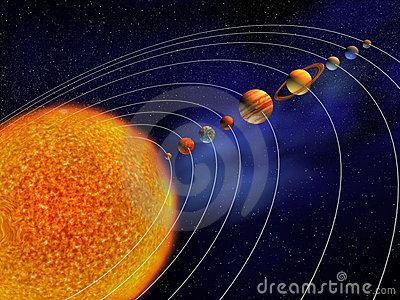
\includegraphics[width=0.45\textwidth]{planetas.jpg}
  \caption{Sistema solar conocido}
  \captionsetup{justification=centering}
  \label{planetas}
\end{figure}
\subsection{Definición de la problemática}
La mayoría de las implementaciones gráficas conocidas muestran simulaciones de la realidad de los planetas y del sistema solar, sus trayectorias, sus lunas o las diferencias entre las velocidades de rotación de cada uno; pero ¿que sucedería si las órbitas de los planetas aumentara y sumados al aumento de la masa del sol, este atrajera a todos los planetas existentes en el sistema conocido?, el fin de el sol y de los planetas como los conocemos es lo que se desea implementar.\\
Skybox es una tecnica que permite que una escena se vea más grande y más impresionante, envolviendo al usuario con una textura que es posible apreciar en una cámara de 360$^{\circ}$\cite{skybox2}.
\begin{figure}[h!]
  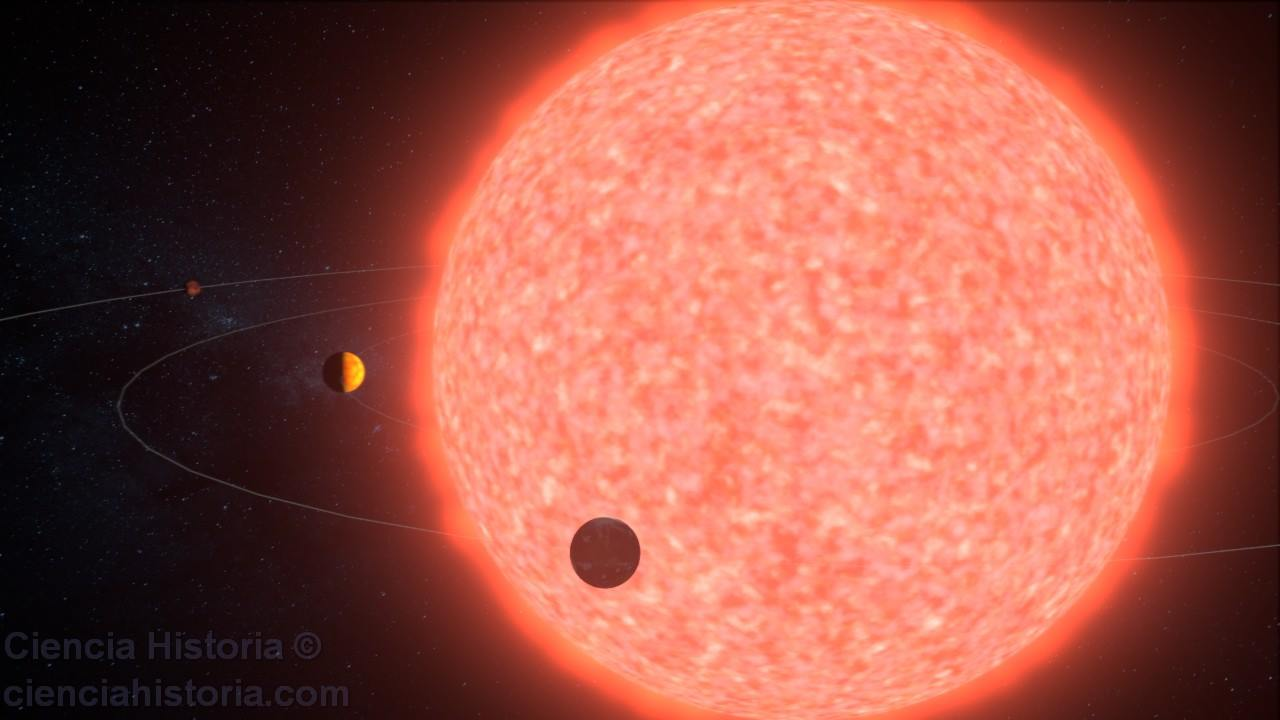
\includegraphics[width=0.48\textwidth]{sol.jpg}
  \caption{El Sol convertido en gigante roja llegando casi a la órbita de Venus, la Tierra tiene un futuro incierto}
  \captionsetup{justification=centering}
  \label{muerte}
\end{figure}
\section{Descripción de la solución propuesta}
Tomando como base el proyecto que solo muestra una representación del sistema solar, se pretende que la representación de las trayectorias de los planetas sea automática, con esto se refiere a que se vea el movimiento continuo de la trayectoria de los planetas y que eventualmente de a poco los planetas comiencen a cambiar su trayectoria, los cuales sumados al aumento del diámetro del sol, como se muestra en \ref{muerte}, empiecen a ser absorbidos por este, lo cual los hará desaparecer\cite{far}.\\
Para ello habría que:
\begin{itemize}
 \item Modificar algunas funciones relacionadas con la traslación de estas diferentes figuras (diferentes planetas)
 \item Editar y acondicionar las formulas de elipse.
 \item Aumentar el radio del sol.
\end{itemize}   %funcion %imagen de traslacion de planetas
\section{Modelamiento}
\subsection{Función de la elipse}
A continuación en la figura \ref{Elipse} se puede ver una elipse para posteriormente analizar su función matemática:

\begin{figure}[h!]
  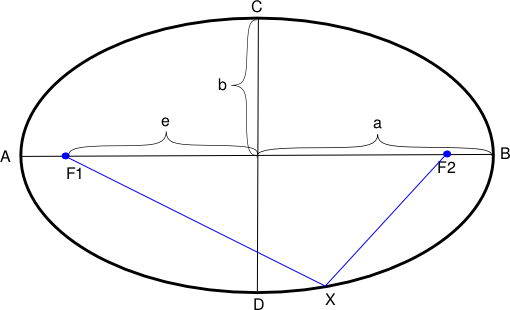
\includegraphics[width=0.48\textwidth]{Elipse.png}
  \caption{Elipse}
  \captionsetup{justification=centering}
  \label{Elipse}
\end{figure}

Se utiliza la función de la elipse:
\begin{huge}
\begin{center}
$\frac{x^{2}}{a^{2}} + \frac{y^{2}}{b^{2}}$
\end{center}
\end{huge}
Donde $a>0$ y $b>0$, las coordenadas de las abscisas. La elipse se encuentra centrada en el origen (h, k = 0). La ecuación de la elipse modela la ubicación de la órbita de los planetas.
\subsection{Transformaciones 3d}
Se utilizan una serie de trasnformaciones en el desarrollo del problema, estas seran mostradas a continuación:
\subsubsection{Rotación}
Claramente como se desea implementar un sistema solar, un detalle importante a destacar es la rotación que tiene cada planeta; la rotación está definida por la siguiente matriz:
\begin{center}
$
\begin{bmatrix}
cos\theta & -sin\theta \\
sin\theta & cos\theta 
\end{bmatrix}
$
\end{center}
En vista de que se trabaja en tres dimensiones es necesario definir las matrices para cada tipo de rotación que se pueden obtener desde la matriz de rotacion general de 2x2:\\
Rotación sobre el eje x:\\
\[
	R_{xy}(\theta) = \left[ 
		\begin{array}{cccc}
			1 & 0 & 0 & 0 \\
			0 & \cos\theta & -\sin\theta & 0 \\
			0 & \sin\theta & \cos\theta & 0 \\
			0 & 0 & 0 & 1
		\end{array}
	\right]
\]
Rotación sobre el eje y:\\
\[
	R_{yz}(\theta) = \left[ 
		\begin{array}{cccc}
			\cos\theta & 0 & \sin\theta & 0 \\
			0 & 1 & 0 & 0 \\
			-\sin\theta & 0 & \cos\theta & 0 \\
			0 & 0 & 0 & 1
		\end{array}
	\right]	
\]
Rotación sobre el eje z:\\
\[
	R_{zx}(\theta) = \left[ 
		\begin{array}{cccc}
			\cos\theta & -\sin\theta & 0 & 0 \\
			\sin\theta & \cos\theta & 0 & 0 \\
			0 & 0 & 1 & 0 \\
			0 & 0 & 0 & 1
		\end{array}
	\right]	
\]

Se describe como rotación en los planos $xy$, $yz$ y $zx$, pues resulta más fácil asociar la rotación en 3 dimensiones de esa forma. La órbita de los planetas se genera aplicando una rotación sobre el eje $y$ (En el origen, teniendo el solo como referencia) con un ángulo $0^{\circ}\leq\theta\leq360^{\circ}$, el cual aumenta en cada frame de la escena.
\subsubsection{Traslación}
La matriz que describe la traslación de los objetos en la escena es la siguiente:\\

\[ 
	T = \left[ 
			\begin{array}{cccc}
				1 & 0 & 0 & T_{x} \\
				0 & 1 & 0 & T_{y} \\
				0 & 0 & 1 & T_{z} \\
				0 & 0 & 0 & 1 
			\end{array}
		\right] \times 
		\left[ 
			\begin{array}{c}
				v_{x} \\
				v_{y} \\
				v_{z} \\
				v_{w} 
			\end{array}
		\right] = 
		\left(
			\begin{array}{ccc}
				v'_{x} , & v'_{y} , & v'_{z}
			\end{array}
		\right)
\]
La traslación permite saber el radio que tendrá la órbita del planeta respecto al sol. Es en torno a esta transformación que se aplica la rotación, por lo tanto para cada frame de la escena se aplica un pequeño aumento en la rotación respectiva.\\
\subsection{Distancia entre dos puntos}
Esta fórmula se utiliza para determinar la distancia entre 2 puntos en un plano en 2D, aunque el sistema está representado en 3 dimensiones. Los planetas se mueven respecto al eje y y la posición de los mismos está determinada sólo por sus coordenadas en el eje x y en el eje z:\\
\[ 
	x_{new} = \frac{\sqrt{X_{final}^{2}+X_{inicial}^{2}}}{100} 
\]
\newline
\[
	z_{new} = \frac{\sqrt{Z_{final}^{2}+Z_{inicial}^{2}}}{100}
\]
\newline
la distancia total entre el punto final y el inicial es dividida por un número random con ello se genera la traslación de un objeto desde un punto hacía otro; lo que se traslada es la viewport
\section{Diseño del problema}

\subsection{Diseño preliminar}

\subsection{Diseño detallado}

\section{Metodología y herramientas a utilizar}
\subsection{Metodología}
La metodología a utilizar es el análisis y diseño estructurado ya que con esta metodología se tiene un orden lógico en los pasos a seguir para el desarrollo correcto del proyecto.
\subsection{Herramientas}
Preliminarmente se tienen las siguientes herramientas para el desarrollo:
\subsubsection{Equipos}
Se posee 2 notebooks con similares características, procesadores Intel core I3 y I5, CPU de 2.4 GHz, 8 Gb de memoria Ram y distribución de Linux Ubuntu 14.04 LTS.
\subsubsection{Herramientas de programación}
Preliminarmente se establecen las siguientes herramientas para la programación, tales como:
\begin{itemize}
 \item Netbeans IDE 8.0.2\\
 	Entre algunas cosas destaca la rapida observación de errores sintaxicos y fácil compilación.
 \item OpenGL\\
 	Principal entorno de desarrollo, para la creación de aplicaciones gráficas portátiles e interactivas en
 	2D y 3D \cite{opengl}.
\end{itemize}
\section{Análisis de resultados}
\subsection{Validación de resultados}
Como se especificó en  la presentación preliminar de la idea, para realizar esta aplicación se toma como base un proyecto anterior del ramo de computación gráfica, el cual se llama "Representación del sistema solar en OpenGL". De este codigo se toman las funciones principales para generar la representacion y se eliminan funciones que no son utilizadas como las que representan estrellas específicas, etc. En el codigo se representa Plutón que no se encontraba representado y además se comienza generando todos los planetas alineados tras el Sol para mantener un orden mas lógico en un principio.
\subsection{Rendimiento preliminar}
En esta etapa de prototipado del proyecto, el equipo de trabajo se enfoca en implementar las funciones más importantes del proyecto base además de aprender sobre la utilización de la herramienta OpenGL. A la base tomada para el desarrollo se le eliminan una serie de funciones que en realidad no serán necesarias por lo tanto esto entregara un código mas compacto y fácil de comprender.\\
Preliminarmente no se identifican problemas relacionados a la presentación en pantalla de la aplicación al ser ejecutada, la velocidad de movimiento (rotación) es más que suficiente para identificar los movimientos de los planetas.\\
\subsection{Problemáticas y funciones faltantes}

\section{Plan de Trabajo}
Se realiza una carta Gantt para darle fechas limites a cada tarea que este proyecto conlleva. Se adjunta para no entorpecer el modelo de este documento y para que la carta Gantt se pueda analizar de mejor manera.
% needed in second column of first page if using \IEEEpubid
%\IEEEpubidadjcol

% An example of a floating figure using the graphicx package.
% Note that \label must occur AFTER (or within) \caption.
% For figures, \caption should occur after the \includegraphics.
% Note that IEEEtran v1.7 and later has special internal code that
% is designed to preserve the operation of \label within \caption
% even when the captionsoff option is in effect. However, because
% of issues like this, it may be the safest practice to put all your
% \label just after \caption rather than within \caption{}.
%
% Reminder: the "draftcls" or "draftclsnofoot", not "draft", class
% option should be used if it is desired that the figures are to be
% displayed while in draft mode.
%
%\begin{figure}[!t]
%\centering
%\includegraphics[width=2.5in]{myfigure}
% where an .eps filename suffix will be assumed under latex, 
% and a .pdf suffix will be assumed for pdflatex; or what has been declared
% via \DeclareGraphicsExtensions.
%\caption{Simulation Results.}
%\label{fig_sim}
%\end{figure}

% Note that IEEE typically puts floats only at the top, even when this
% results in a large percentage of a column being occupied by floats.
% However, the Computer Society has been known to put floats at the bottom.


% An example of a double column floating figure using two subfigures.
% (The subfig.sty package must be loaded for this to work.)
% The subfigure \label commands are set within each subfloat command,
% and the \label for the overall figure must come after \caption.
% \hfil is used as a separator to get equal spacing.
% Watch out that the combined width of all the subfigures on a 
% line do not exceed the text width or a line break will occur.
%
%\begin{figure*}[!t]
%\centering
%\subfloat[Case I]{\includegraphics[width=2.5in]{box}%
%\label{fig_first_case}}
%\hfil
%\subfloat[Case II]{\includegraphics[width=2.5in]{box}%
%\label{fig_second_case}}
%\caption{Simulation results.}
%\label{fig_sim}
%\end{figure*}
%
% Note that often IEEE papers with subfigures do not employ subfigure
% captions (using the optional argument to \subfloat[]), but instead will
% reference/describe all of them (a), (b), etc., within the main caption.


% An example of a floating table. Note that, for IEEE style tables, the 
% \caption command should come BEFORE the table. Table text will default to
% \footnotesize as IEEE normally uses this smaller font for tables.
% The \label must come after \caption as always.
%
%\begin{table}[!t]
%% increase table row spacing, adjust to taste
%\renewcommand{\arraystretch}{1.3}
% if using array.sty, it might be a good idea to tweak the value of
% \extrarowheight as needed to properly center the text within the cells
%\caption{An Example of a Table}
%\label{table_example}
%\centering
%% Some packages, such as MDW tools, offer better commands for making tables
%% than the plain LaTeX2e tabular which is used here.
%\begin{tabular}{|c||c|}
%\hline
%One & Two\\
%\hline
%Three & Four\\
%\hline
%\end{tabular}
%\end{table}


% Note that IEEE does not put floats in the very first column - or typically
% anywhere on the first page for that matter. Also, in-text middle ("here")
% positioning is not used. Most IEEE journals use top floats exclusively.
% However, Computer Society journals sometimes do use bottom floats - bear
% this in mind when choosing appropriate optional arguments for the
% figure/table environments.
% Note that, LaTeX2e, unlike IEEE journals, places footnotes above bottom
% floats. This can be corrected via the \fnbelowfloat command of the
% stfloats package.





\section{Conclusiones}

Como inicio para un buen proyecto, siempre se deben llevar a cabo investigaciones que puedan determinar cual tema abordar y que herramientas utilizar para un optimo desempeño durante este.\\
El tema abordado nos llena de optimismo para trabajar en el, sumado a los conceptos de computación gráfica aprendidos más la investigación pertinente, nos motiva a dar el 100\% de nuestro esfuerzo para hacer de este un gran proyecto.

% trigger a \newpage just before the given reference
% number - used to balance the columns on the last page
% adjust value as needed - may need to be readjusted if
% the document is modified later
%\IEEEtriggeratref{8}
% The "triggered" command can be changed if desired:
%\IEEEtriggercmd{\enlargethispage{-5in}}

% references section

% can use a bibliography generated by BibTeX as a .bbl file
% BibTeX documentation can be easily obtained at:
% http://www.ctan.org/tex-archive/biblio/bibtex/contrib/doc/
% The IEEEtran BibTeX style support page is at:
% http://www.michaelshell.org/tex/ieeetran/bibtex/
%\bibliographystyle{IEEEtran}
% argument is your BibTeX string definitions and bibliography database(s)
%\bibliography{IEEEabrv,../bib/paper}
%
% <OR> manually copy in the resultant .bbl file
% set second argument of \begin to the number of references
% (used to reserve space for the reference number labels box)

\bibliographystyle{IEEEtran}
\bibliography{bibi}
% that's all folks
\end{document}

